\documentclass{article}

\usepackage{graphicx}
\usepackage{tikz}
\usepackage{tikzsymbols}
\usetikzlibrary{calc,patterns,shapes.geometric}
\pagestyle{empty}
\usepackage[margin=0pt]{geometry}
\geometry{papersize={14in,12in}}

\def\centerarc[#1](#2)(#3:#4:#5){\draw[#1] ($(#2)+({#5*cos(#3)},{#5*sin(#3)})$) arc (#3:#4:#5);}

\begin{document}
	\begin{figure}
		\centering
		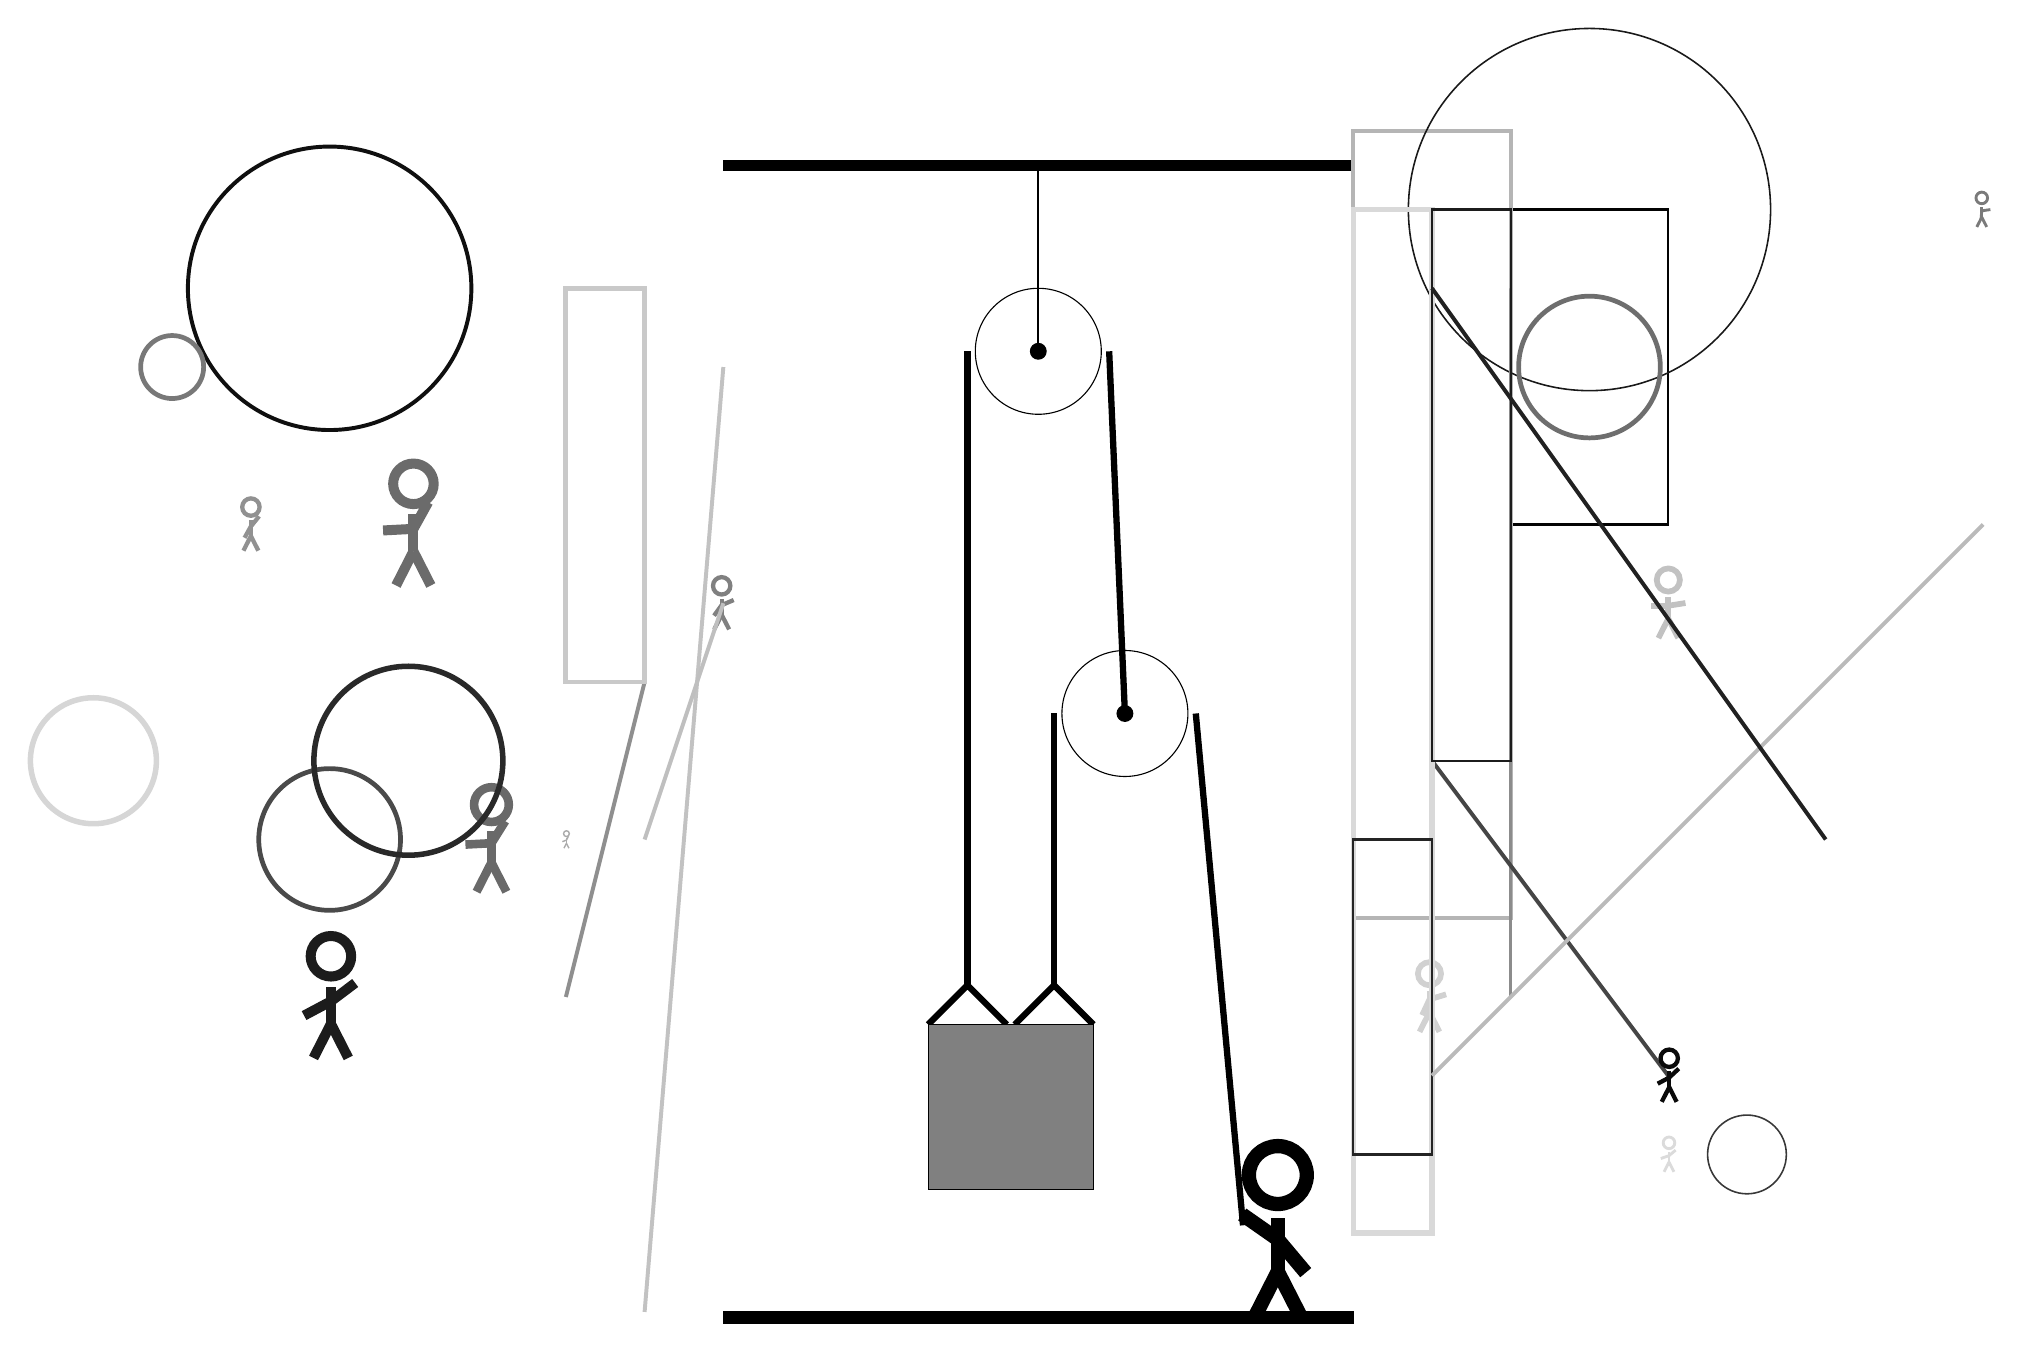
\begin{tikzpicture}
			%%%%% START %%%%%
			
			\draw[fill=black] (-2, 11.5) rectangle (6, 11.625);
			
			\draw (2, 9.2) circle (0.8);
			\draw[fill=black] (2, 9.2) circle (0.1);
			\draw[thick] (2, 9.2) -- (2, 11.5);
			
			\draw (3.1, 4.6) circle (0.8);
			\draw[fill=black] (3.1, 4.6) circle (0.1);
			
			\draw[line width = 0.8mm]  (0.6, 0.65) -- (1.1, 1.15) -- (1.6, 0.65);
			\draw[line width = 0.8mm]  (1.7, 0.65) -- (2.2, 1.15) -- (2.7, 0.65);
			\draw[fill=black!50] (0.6, 0.65) rectangle (2.7, -1.45);
			
			\draw[line width = 0.8mm] (1.1, 9.2) -- (1.1, 1.15);
			\centerarc[line width = 0.8mm](2, 9.2)(0:180:0.9);
			\draw[line width = 0.8mm] (2.9, 9.2) -- (3.1, 4.6);
			\draw[line width = 0.8mm] (2.2, 4.6) -- (2.2, 1.15);
			\centerarc[line width = 0.8mm](3.1, 4.6)(0:180:0.9);
			\draw[line width = 0.8mm] (4.0, 4.6) -- (4.6, -1.9);
			
			\node at (5, -2) {\Strichmaxerl[10][-35][-50]};
			
			\node[line width=0.5mm, color=black!24] at (10, 6) {\Strichmaxerl[4][0][9]};
			
			\draw[line width=0.5mm, color=black!44](-4, 1) -- (-3, 5);
			\draw[line width=0.3mm, color=black!99] (8, 7) rectangle (10, 11);
			\draw[line width=0.5mm, color=black!29] (6, 2) rectangle (8, 12);
			\draw [line width=0.2mm, color=black!90](9, 11) circle (2.3);
			
			\draw[line width=0.4mm, color=black!45] (8, 10) rectangle (8, 1);
			
			\draw [line width=0.6mm, color=black!71](-7, 3) circle (0.9);
			
			\node[line width=0.5mm, color=black!59] at (-5, 3) {\Strichmaxerl[6][3][58]};
			\draw[line width=0.6mm, color=black!21] (-3, 5) rectangle (-4, 10);
			\draw [line width=0.6mm, color=black!57](9, 9) circle (0.9);
			
			\draw[line width=0.5mm, color=black!73](7, 4) -- (10, 0);
			
			\node[line width=0.3mm, color=black!18] at (7, 1) {\Strichmaxerl[4][65][17]};
			\draw[line width=0.7mm, color=black!15] (7, -2) rectangle (6, 11);
			\draw[line width=0.3mm, color=black!86] (7, -1) rectangle (6, 3);
			\draw[line width=0.5mm, color=black!24](-3, -3) -- (-2, 9);
			\draw [line width=0.5mm, color=black!94](-7, 10) circle (1.8);
			
			\node[line width=0.7mm, color=black!58] at (-6, 7) {\Strichmaxerl[7][3][61]};
			
			\draw [line width=0.7mm, color=black!16](-10, 4) circle (0.8);
			\draw[line width=0.5mm, color=black!27](7, 0) -- (14, 7);
			\node[line width=0.4mm, color=black!43] at (-8, 7) {\Strichmaxerl[3][61][51]};
			\draw[line width=0.3mm, color=black!89] (8, 11) rectangle (7, 4);
			\draw [line width=0.2mm, color=black!78](11, -1) circle (0.5);
			\draw [line width=0.6mm, color=black!53](-9, 9) circle (0.4);
			\node[line width=0.4mm, color=black!50] at (-2, 6) {\Strichmaxerl[3][54][23]};
			\node[line width=0.2mm, color=black!33] at (-4, 3) {\Strichmaxerl[1][21][63]};
			\node[line width=0.7mm, color=black!96] at (10, 0) {\Strichmaxerl[3][28][43]};
			\draw[line width=0.5mm, color=black!87](7, 10) -- (12, 3);
			\draw [line width=0.7mm, color=black!84](-6, 4) circle (1.2);
			\node[line width=0.6mm, color=black!52] at (14, 11) {\Strichmaxerl[2][85][8]};
			
			\node[line width=0.5mm, color=black!89] at (-7, 1) {\Strichmaxerl[7][28][37]};
			\node[line width=0.2mm, color=black!14] at (10, -1) {\Strichmaxerl[2][19][40]};
			
			\draw[line width=0.5mm, color=black!25](-2, 6) -- (-3, 3);
			
			\draw[fill=black] (-2, -3) rectangle (6, -3.15);
			
			%%%%% END %%%%%
		\end{tikzpicture}
	\end{figure}	
\end{document}